\section{Delsystem}

Systemet är indelat i två olika delsystem. Dessa system kommer köras
sekvensiellt, alltså det ena efter det andra. Det första systemet kontrollerar
själva bilkörningen medan det andra systemet kontrollerar displayen. Se
figur~\ref{fig:system_diagram} för ett processchema.

\begin{figure}
  \centering
  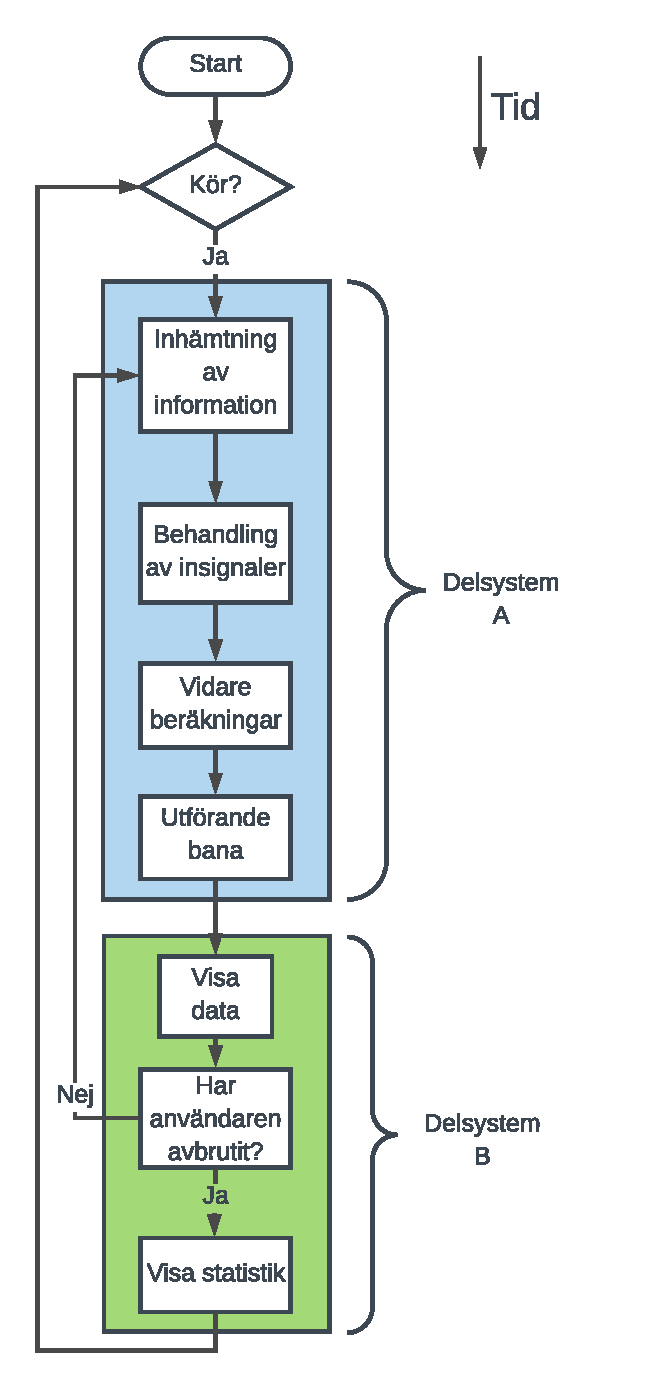
\includegraphics[width=\linewidth]{figures/Processchema.pdf}
  \caption{Processchema över systemets helhet.}%
  \label{fig:system_diagram}
\end{figure}

  \subsection{Delsystem A: Bana}
  
  Delsystem A är indelat i tre övergripande delar. I del A.1 hämtas all
  tillgänglig information in, i del A.2a görs beräkningar utifrån tillgänglig
  data, i del A.2b görs vidare beräkningar (alltså beräkningar som inte baseras
  direkt på den tillgängliga informationen), och i del A.3 utförs de ändringar
  som programmet bedömer är nödvändiga för att klara den valda varvtiden. 

    \subsubsection{Inhämtning av information}

    Information som finns tillgänglig är kraftigt begränsad. I praktiken kommer
    programmet endast fråga om någon av bilarna passerat en givare sedan
    programmet frågade förra gången.

    \subsubsection{Primära beräkningar}

    De primära beräkningarna är de beräkningar som beror direkt på tillgänglig
    information. Eftersom indatan enbart består av bilens position är bilens
    hastighet genom det förra segmentet den enda informationen som direkt beror
    på indata.

    \subsubsection{Sekundära beräkningar}
    
    Den första beräkningen som görs är bilens nuvarande position. Detta görs med
    hjälp av en intern bild av banan och vetskapen om vilken hastighet bilen
    önskas ha. Sedan räknas den position som bäst gör att bilen klarar den satta
    varvtiden ut. För att räkna ut den beaktas enbart den nuvarande tiden och
    (om gemensam målgång är aktiverat) positionen av den andra bilen. Steget
    efter är att räkna ut den mest rimliga optimala situationen som beaktar hur
    lång tid det är kvar på det nuvarande varvet. I början av varvet görs alltså
    inte lika drastiska hastighetsändringar som mot slutet.

    Det sista som händer är när informationen om bilens och banans skick används
    för att räkna ut vilket spänningspådrag som krävs för att få bilen att nå
    den hastighet och position som krävs.

    \subsubsection{Utförande}

    I utförandet skickas det nya spänningspådraget till banorna. 
	

    \subsubsection{Funktioner i delsystem A} \label{sec:system_a_funcs}
    I figur~\ref{fig:flow_diagram}  visas flödet av de funktioner som sker i delsystem A under en cykel.
    Här listas namn på funktionerna och deras funktion:
    \begin{itemize}
      \item indata: Ger data när bilen passerar en givare.
      \item car constant: Programmets sätt att anpassa sig efter olika bilars egenskaper. Justeras vid varje ny indata.
      \item position: Där programmet tror att bilen är.
      \item clock: Hur länge bilen har varit i det nuvarande segmentet och varvet.
      \item car position dif: Bilarnas position relativt till varandra. Endast aktiv om gemensam målgång aktiverad.
      \item target: Den varvtid som manuellt har satts inan programet startade.
      \item target dif: Bilens position relativt till var den borde vara vid den nuvarande tiden.
      \item agressivness: Hur bråttom det är att justera bilarnas hastighet.
      \item u constant map: En ``karta'' över hur mycket spänning som behövs i olika delar av banan.
      \item track u constant: Konstant för att justera spänningen på nuvarande position.
      \item speed map: En ``karta'' över hur fort man kan köra i olika delar av banan.
      \item speed constant: Konstant som används för att se till att hastigheten anpassas efter banans svängar m.m.
      \item new v: Den nya hastigheten som ska sättas.
      \item new u: Den spänning som skickas till bilen.
    \end{itemize}

    \begin{figure}
      \centering
      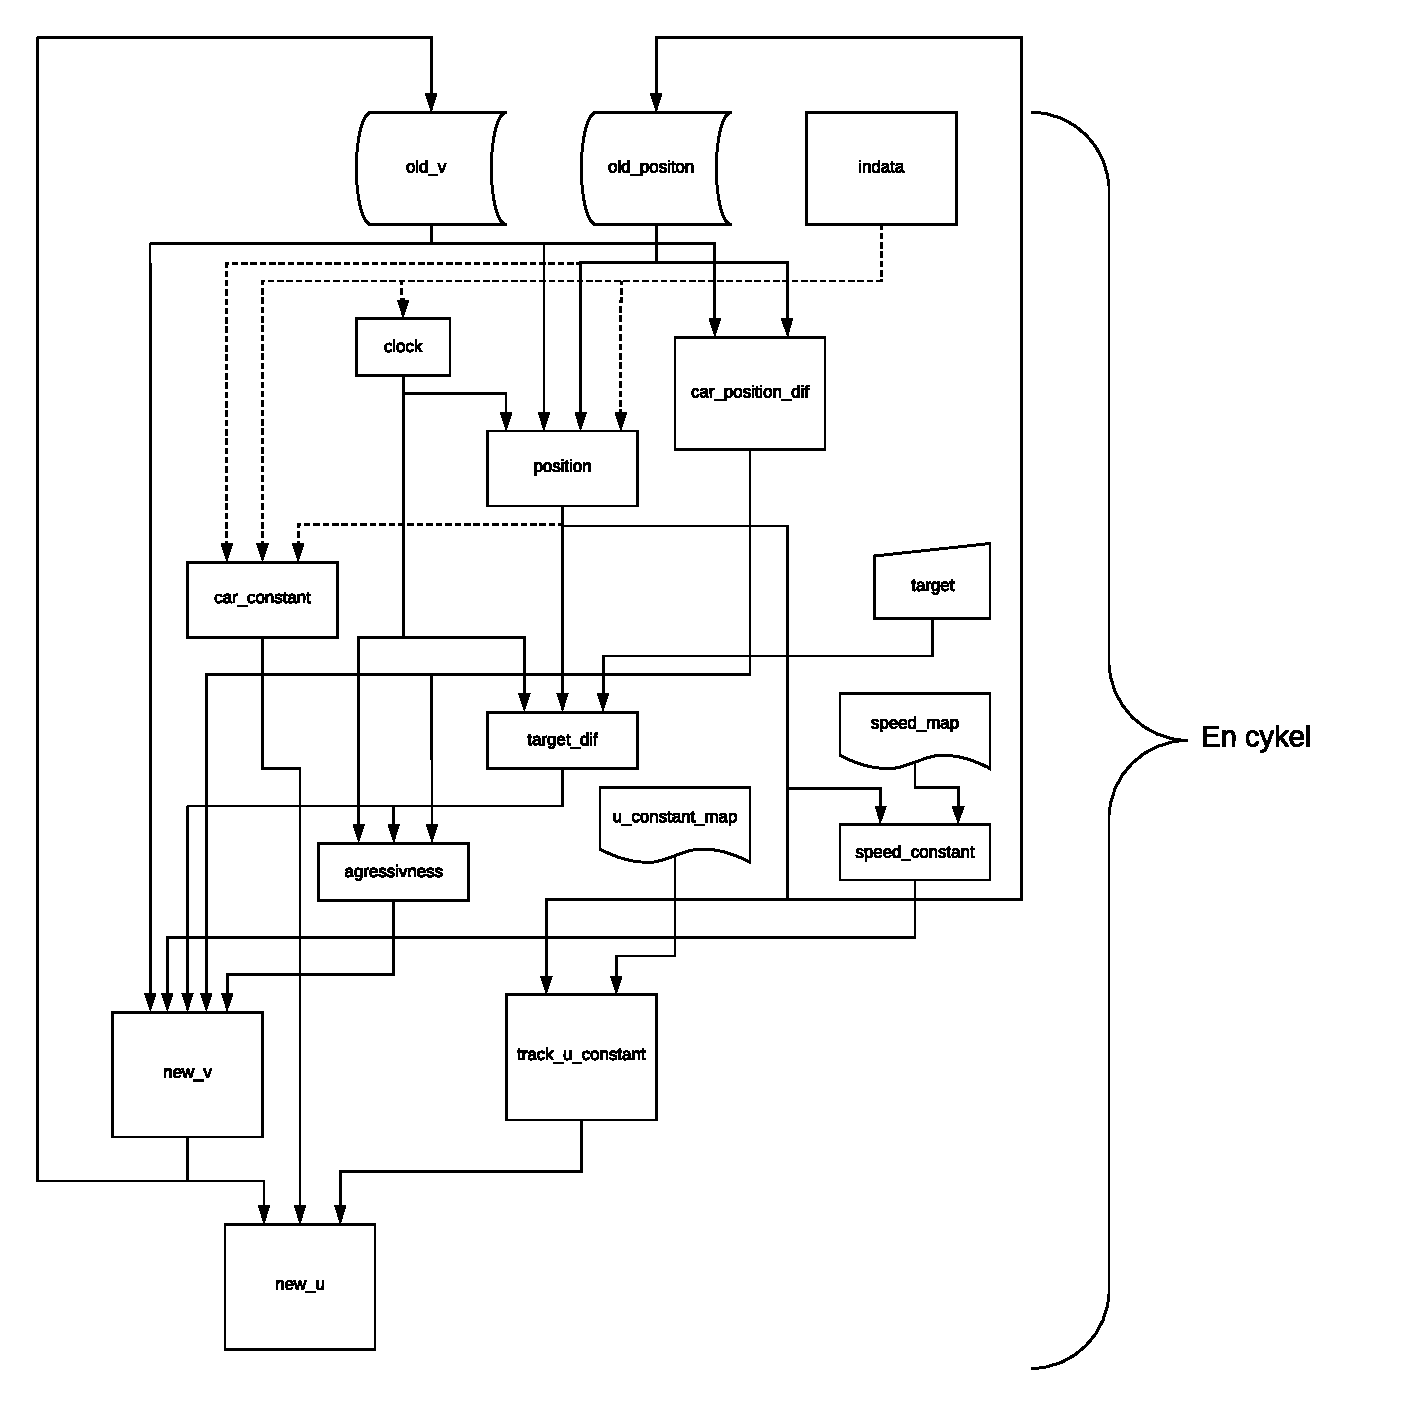
\includegraphics[width=\linewidth]{figures/flow.pdf}
      \caption{Funktionsflödet i delsystem A.}%
      \label{fig:flow_diagram}
    \end{figure}

  \subsection{Delsystem B: Display}

  Displayen ter sig enklare än delsystem A. Under körning ska, om ett nytt varv
  påbörjats, den senaste varvtiden och varvnumret skickas till displayen. Om
  stopp-knappen har tryckts ned ska systemet hoppa till resultat-skärmen och om
  inte så ska det fortsätta.

